\documentclass[a4paper,10pt, twocolumn]{article}
\usepackage{amsmath}
\usepackage{graphicx}
\usepackage[font={small,it}]{caption}
\usepackage{multirow}
\usepackage{algpseudocode,algorithm,algorithmicx}
\newcommand*\DNA{\textsc{dna}}
\usepackage[]{mcode}

\newcommand*\Let[2]{\State #1 $\gets$ #2}
\algrenewcommand\algorithmicrequire{\textbf{Precondition:}}
\algrenewcommand\algorithmicensure{\textbf{Postcondition:}}

\begin{document}

\title{Efficient frontier and portfolio optimisation}
\author{Alun Meredith}
\maketitle

\section{Introduction}
The modern era of portfolio management was brought about by the concept of the efficient frontier by Harry Markowitz (1952) \cite{Portfolio}. Markowitz describes that along with maximising returns, minimising risk is also important. To this end he proposes the Mean-Variance Frontier, a set of Pareto optimal portfolios. I.e. for any given return it risk cannot be reduced and vice versa.   

In order to construct this boundary stock price is modelled as normally distributed with a mean, $r$ (expected return) and variance, $v$ (risk/volatility). Short selling is also discounted to give the two additional constraints for portfolios: $w \geq 0$ and $\mathbf{w^T1} = 1$.  

Under these conditions the frontier portfolios can be found by solving the linear problem:

\begin{align}
 max_w \  \mathbf{w^Tr} \  subject \  to \  \mathbf{r^TCr} = \sigma_0 
 \label{eq:return}
\end{align}

In order to find the maximum return for any given variance, or for a given expected return minimise risk by solving the quadratic problem:

\begin{align}
 min_w \ \mathbf{w^TCw} \ subject \  to \  \mathbf{w^Tr} = r_0
 \label{eq:var}
\end{align}

Since 1952 there have been a number of criticisms of this mean-variance model. Firstly under the assumptions made modelling stocks as normally distributed. Stock prices do not always fluctuate in this manor and covariances are not always constant, especially in the situation of a crash. This means that the returns and covariances of stocks must be estimated when predicting the future.  

A second criticism is that although the mean-variance frontier performs well when we the return and risk are known (retrospective), it is extremely volatile to fluctuations\cite{VsNaive}. This large impact of estimation error makes it very difficult to construct portfolios which perform better than a naive diversified approach. 

In the last decade some work has been made to try to address some of these issues making adjustments to the model in order to construct more robust portfolios and model additional constraints such as transaction costs \cite{Regularisation}. 

The structure is as follows: In the next section look at the Mean-Variance frontier and explore the performance of different algorithms which compute it. Then we consider the performance of portfolios on the frontier on data from the last 3 years of the FTSE-100, comparing it to a naive approach. In section 4 we include the modelling of fixed transaction costs and using both a greedy algorithm and lasso regularisation to approximate the FTSE-100 index. Finally we look at modelling linear transaction costs and how other constraints can be built on top of the Efficient Frontier model. 

\section{Mean-Variance Frontier}
In this section we explore the mean-variance space and the efficient frontier before comparing three diffierent algorithms for computing the efficient frontier: Matlab\'s Portfolio optimisation through the Financial Toolbox package \cite{Matlab} and the NaiveMW algorithm developed by described by P. Brandimarte \cite{TextBook}, using both linprog/quadprog and CVX \cite{CVX} to compute the optimisation steps.  

Test data is given by three artificial assets (taken from example in MATLAB's Finance Toolbox) whose expected returns and covariances are:
\begin{align}
r &= 
  \begin{bmatrix}
  0.10 \\ 0.20 \\ 0.15
  \end{bmatrix} 
C &=
  \begin{bmatrix}
     0.005 & -0.010 &  0.004 \\
    -0.010 &  0.040 & -0.002 \\
     0.004 & -0.002 & -0.023
  \end{bmatrix}
  \label{eq1}
\end{align}


\begin{figure*}[t]
	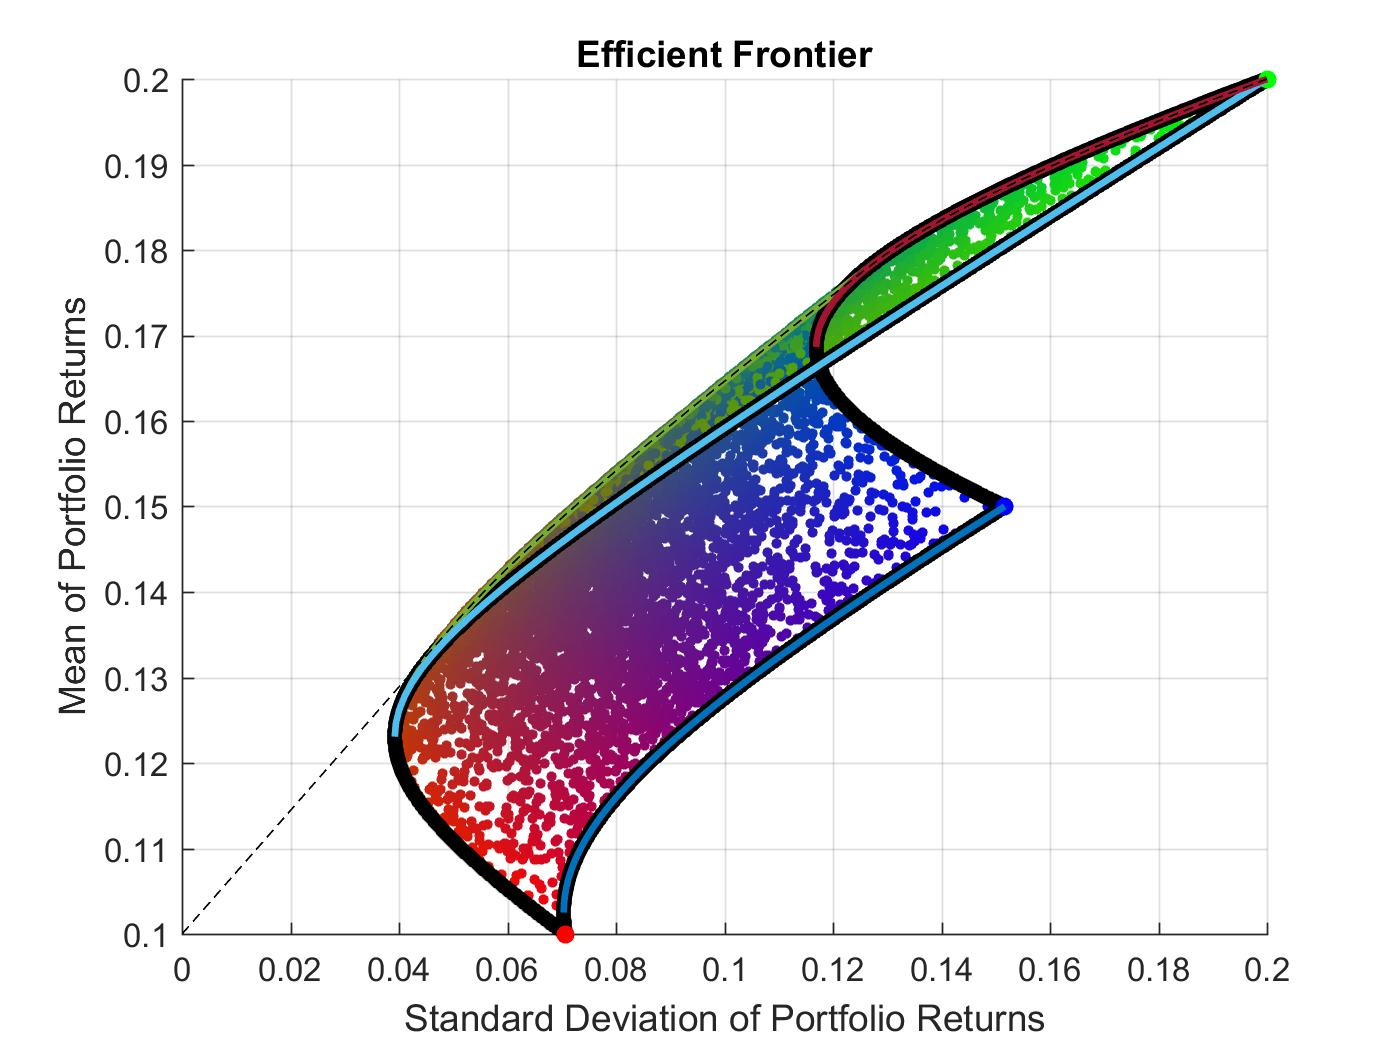
\includegraphics[width=\textwidth]{EVspace.jpg}
	\centering
	\caption{E-V space of 10000 samples of portfolios generated from the 3 assets shown in equation \ref{eq1}. RGB values of points shows the distribution of weights across each asset: 1-Red, 2-Blue, 3-Green. Singular portfolios shown by large points. Black lines between singular assets show pairwise portfolio samples of those two assets. Coloured lines show efficient frontiers of each combination of asset computed using Matlab's financial toolbox: 1\&2-Cyan, 2\&3-Red, 1\&3-Blue, 1\&2\&3-Green. Dashed line shows efficient frontier with the inclusion of risk-less asset.}
			\label{fig:EVspace}
\end{figure*} 

The efficient frontier is outer limit of E-V space from the minimum variance point to the maximum return point. The frontier includes mixtures of all three assets; this ranges from 1\&2 to 2\&3 to 3 as it travels from minimum variance to maximum return. For the pairwise portfolios the frontier simply follows the linear E-V space from these the maxima.

The E-V space (fig. \ref{fig:EVspace}) shows the possible E-V space. The frontier mostly comprised of two asset portfolios (black). The maximum return portfolio is the singular asset 2 portfolio (green), whereas the minimum variance portfolio is a mixture of asset 1 and 2.

For any two assets which are negatively correlated a mixture of the two assets will improve the variance. It is for this reason while the maximum return point is always a singular stock portfolio the minimum variance is usually a mixed asset portfolio. This is demonstrated in the efficient frontiers of the pairwise stock. The pairs which are negatively correlated have optimum variance portfolios, which aren't singular, whereas the positively correlated pairwise does not.

So far only combinations of risky assets have been considered, however investors also have the option of not investing some portion of their money in risky assets and instead keeping them in a risk-less form such as collecting interest in a bank. If a risk-less asset with fixed return, ($m = 0.1$) and no correlation with other assets is considered the Efficient frontier shifts to include a line from the singular risk-less asset portfolio to the tangent of the previous frontier. This tangent line represents the ratio of equity in a the risk-less asset or the risky portfolio. The point where the tangent touches the risky frontier; where the investor is first willing to put all of their assets into a risky portfolio is the pure risky portfolio which maximises the Sharpe ratio. 

The Sharpe ratio is a described as the excess return (return above risk-less return) over the risk (standard deviation of returns). Another performance metric used is Value at Risk, which is value of assets being risked at a set probability.

\begin{align}
S = \frac{r - interest}{\sigma} \\
V  \ such\  that\   P[G < -V] = p_0
\label{eq:sharpe}
\end{align}

Where S is Sharpe ratio, G is gains, V is value at risk and $p_0$ is the probability level given. 


\subsection{Comparing algorithms}

Matlab's portfolio optimisation tools are based on Markowitz portfolio optimisation theory \cite{Portfolio}, however the algorithms used are somewhat of a black box. P. Brandimarte describes \textit{NaiveMW}: "a (very) simplified version of frontcon" \cite{TextBook} where the algorithm is more transparent (algorithm. \ref{alg:NaiveMW}). In recent years, Frontcon has been refactored into the Portfolio function. 

\begin{algorithm}
  \caption{NaiveMW Pseudocode: Computing portfolio weights for efficient frontier \cite{TextBook}
    \label{alg:NaiveMW}}
  \begin{algorithmic}[1]
    \Statex
      \Let{MaxReturn}{maximise(return).return} 
      \Let{MinVarReturn}{minimise(variance).return}
      \Let{ReturnRange}{linspace(MinVarReturn, MaxReturn, N)}
      \For{i = 1:N}
        \Let{FrontierWeights(i,:)}{minimise(variance constrained by ReturnRange(i)} 
      \EndFor
  \end{algorithmic}
\end{algorithm}

The NaiveMW algorithm finds the return range between the minimum variance point and maximum return point (lines 1-3), before minimising the variance for a sequence of points along that range. Maximising return $\mathbf{w^Tr}$ is a linear equation (use linprog); the additive property of return value in the portfolios means the return value is simply the weighted sum of asset return values. However the variance is not additive, the cumulative variance of a portfolio is given by eq. \ref{eq:var}; where $\mathbf{w^TCw}$ is the quadratic form of the covariance matrix (use quadprog). These equations can be derived empirically from the 2-Dimensional Gaussian density. 

\begin{table}[t]
\begin{tabular}{|r|l|l|l|l|}
  \hline
  \# of Assets & \multicolumn{2}{ |c| }{3}  & \multicolumn{2}{ |c| }{2}\\
  \hline
  & Mean & Var & Mean & Var \\
  \hline 
  Portfolio & 0.1160 & 0.169 & 0.0696 & 0.0001 \\
  Naive\_MW & 0.4712 & 0.0460 & 0.4080 & 0.0021 \\ 
  Naive(CVX) & 1.3081 & 0.2682 & 1.1891 & 0.0213 \\
  \hline 
\end{tabular}
\caption{The time taken, in seconds, for each algorithm to compute the efficient frontier of the sample assets (eq. \ref{eq1}). Each combination of assets is repeated 10 times}
\label{table:1}
\end{table}

The portfolio function is significantly computationally quicker than the other two algorithms \ref{table:1} however appears to be impacted by the increased complexity much more, nearly doubling in computing time between the two portfolio sizes tested. It is unclear if this would make the Naive\_MW algorithm faster at high dimensional portfolios or just narrow the gap. The linprog and quadprog functions also are significantly faster than the CVX optimisations. This is possibly a trade-off between computational efficiency and flexibility. The main advantage to CVX is its syntax and legibility as well as its flexibility/adaptability, in section 4 and 5 CVX optimisations are easily adapted to include additional constraints. 

\begin{figure}[t]
	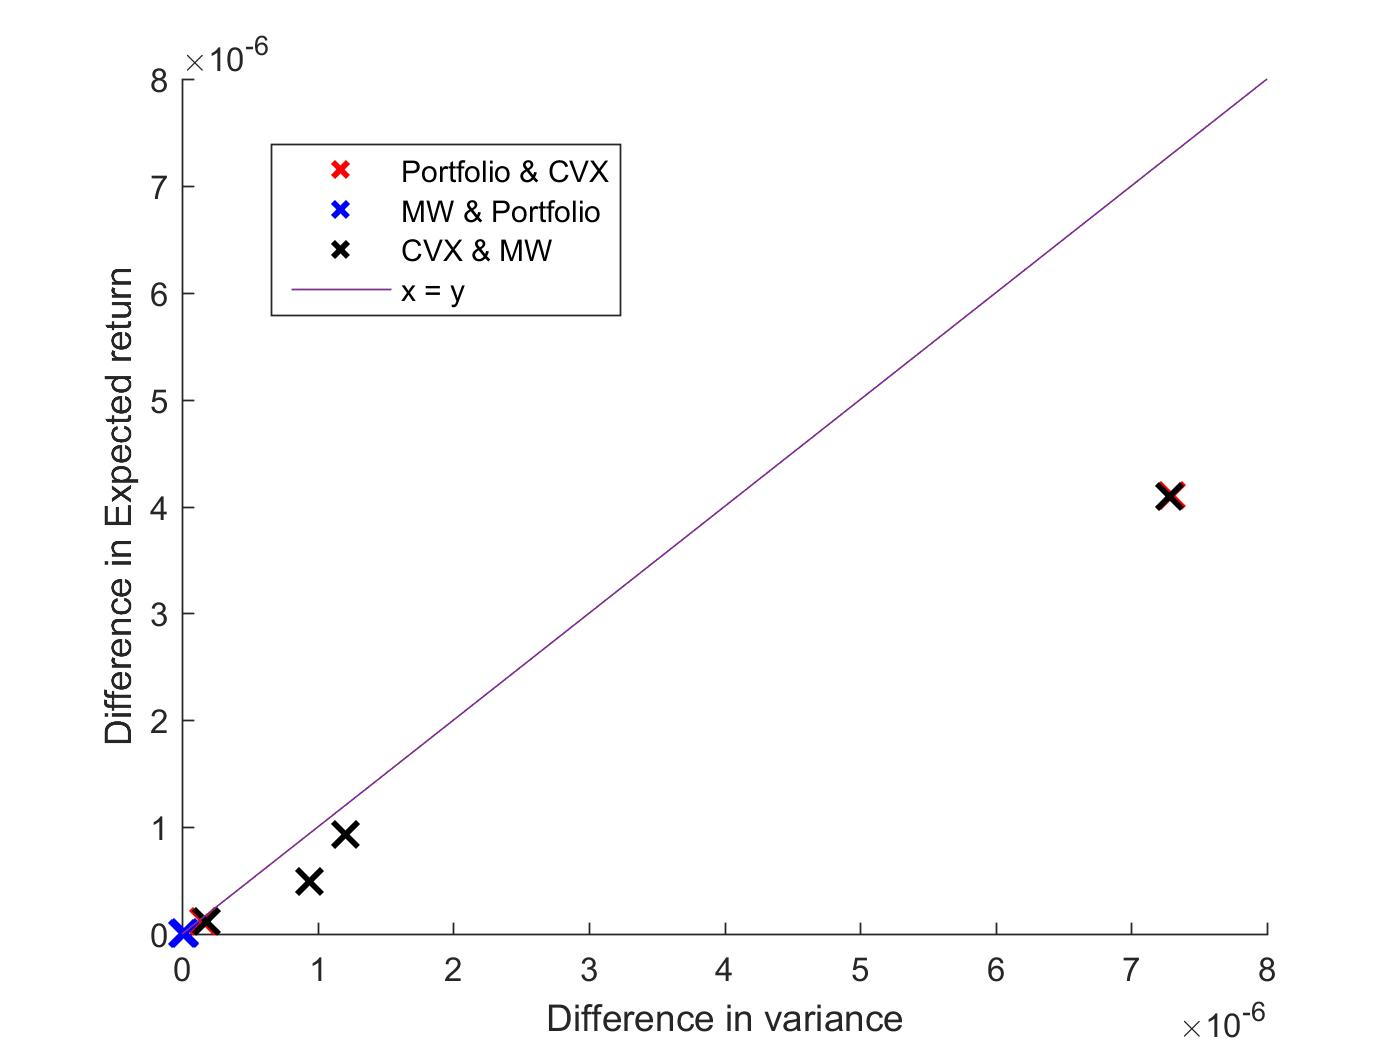
\includegraphics[width=\linewidth]{FrontierDifferences.jpg}
	\centering
	\caption{Pairwise differences in E-V space for Frontier points calculated by the three algorithms. Differences were evaluated 10 times and average taken; Errors are of order $10^{-8}$ so error bars neglected.}
			\label{fig:FrontierDifference}
\end{figure}

Although it is difficult to measure the performance of the different frontiers comparing the differences in weights of points computed on the frontier can help identify how closely the different algorithms compute frontiers to one another (fig. \ref{fig:FrontierDifference}). We can see that the MW and Portfolio algorithms yield the same result. This likely means that underneath Portfolio uses linprog and quadprog in its optimisation steps. CVX produces more variance in its result. However this can be due to computing different points along the frontier. The order of differences is still small enough to consider them roughly equivalent. 

\section{Mean-Variance Vs. Naive}
\begin{table*}[t]
\begin{tabular}{|c|c|l|l|l|l|}
  \hline
  \multirow{ 2}{*}{Portfolio} & \multirow{ 2}{*}{Data} & Return & Var & Sharpe & VaR\\
   & & $10^{-4}$ & $10^{-4}$ & & $10^{-4}$ \\
  \hline 
  \multirow{ 2}{*}{Frontier} & In Sample & $6.60 \pm 0.27$ & $2.15 \pm 0.04$ & $0.044 \pm 0.018$ & $0.75 \pm 0.02$ \\
  & Out of Sample & $6.45 \pm 0.29$ & $2.67 \pm 0.01$ & $0.045 \pm 0.002$ & $1.23 \pm 0.09$\\ 
  \hline  
  \multirow{ 2}{*}{1/N} & In Sample & $0.49 \pm 0.20$ & $1.81\pm0.02$ & $0.006\pm0.002$ & $3.43\pm0.002$ \\
  & Out of Sample & $5.35\pm0.22$ & $1.27\pm0.03$ & $0.049\pm0.002$ & $0.39\pm0.022$ \\
  \hline 
\end{tabular}
\caption{Performance Metrics of Maximum Sharpe Ratio efficient frontier portfolio vs 1/N naive diversified portfolio for a random sample of 3 stocks in the FTSE 100 index. Confidence intervals are show a 95\% sample error.}
\end{table*}

We consider the past 3 years of FTSE-100 stocks from 18/02/2013 - 17/02/2013 inclusive, data courtesy of Yahoo finance. The data was first cleaned by removing values listed on days where the market was known to be closed, weekends and holidays. Any stock for which there were more than 5\% missing values were removed, this was usually due to that company entering the FTSE-100 some time in the last 3 years. Removing these companies also helps restrict the bias we have for selecting companies which are still in the FTSE after 3 years (companies which did sufficiently poorly over this time would have left the index). Finally any remaining missing values were imputed in two ways: in one case the missing values were all at the start of the time series, here the average daily change in value for the next month was calculated and then this change was retrofitted backwards; for the other stock the mean value either side of the missing value was imputed. The first half of the time series was taken as a training set while the second half as a testing set. Of the remaining stock a random sample of 30 of them were used in the evaluation to limit performance costs. 

In the previous section the return and covariance of the stocks were known. Here they must be approximated from the training set using the following formulae:

\begin{align}
\hat{r} &= \frac{1}{T}\sum^T_{t=1}r(t) \\
\hat{\sigma}^2 &= \frac{1}{T}\sum^T_{t=1}(r(t)-\hat{r})(r(t)-\hat{r})^T
\label{eq:}
\end{align}

Once estimated the set of efficient portfolios can be computed. Although all portfolios on the efficient frontier are viable candidates, modelling the different levels of tolerated risk, the portfolio with the greatest in-sample Sharpe ratio was tested in order to have a single consistent way of picking a portfolio to test. 

The testing set (8/2015-2/2016) sees significant performance improvements for the 1/N naive portfolio in all measures. As the naive strategy is in-discriminant this reflects an improving general market position. The difference between in-sample and out of sample performance gives a measure of estimation error. While the frontier portfolio reaches high performance levels on the test set it fails to estimate well and the naive approach sees greater Sharpe ratios and lower value at risk although average returns are still low. 

The Sharpe ratio sees modest improvements with the number of stock in the portfolio but the difference between the frontier and naive stock here is fairly constant so it is hard to say that this supports Miguel's hypothesis that low number of assets gives less room for estimation error and leads to the smallest difference between the naive and frontier strategies. The effect of stock size is far greater on the training set than test set for the frontier strategy indicating over-fitting. 


\begin{figure}[ht]
	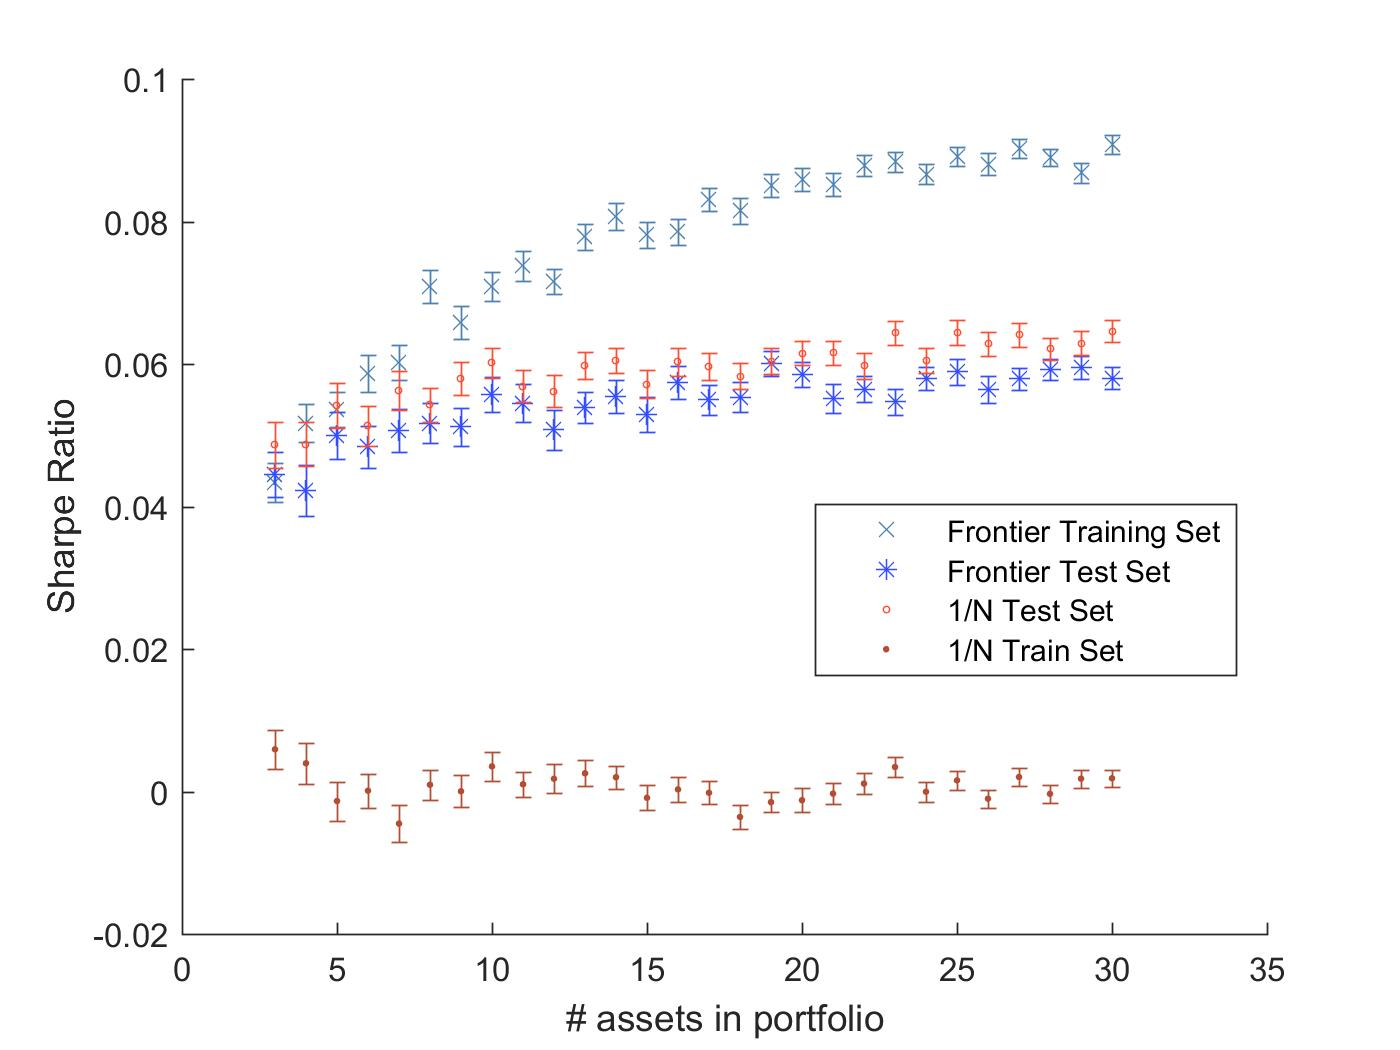
\includegraphics[width=\linewidth]{Sharpe.jpg}
	\centering
	\caption{{Performance of frontier portfolio with greatest Sharpe ratio the last 3 years both in and out of sample versus the naive 1/N portfolio for 100 repetitions while varying the number of assets in the portfolio}}
			\label{fig:Performance_WA}
\end{figure}

Overall these results shows a pattern of overfitting leading to estimation error: a problem commonly dealt with in machine learning with techniques such as regularisation; and greater performance of a naive strategy when using performance metrics which care about variance, this reflects that the strength of its performance comes from the power of diversification on lowering variance.

\section{Index-Tracking}
\begin{table}
\begin{tabular}{|r|c|c|c|c|}
\hline
$10^{-3}$ & \multicolumn{2}{|c|}{Training Set} & \multicolumn{2}{|c|}{Testing Set} \\
\hline
& $\mu$ & $\sigma$ & $\mu$ & $\sigma$ \\
\hline
Greedy & -0.435 & 11.5 & 0.229 & 8.93\\
\hline
Lasso & 0.087 & 12.4 & 0.570 & 9.29\\
\hline
\end{tabular}
\caption{Average error in return between FTSE-100 index and low cardinality portfolios constructed by either greedy algorithm or lasso regression using a random sample of 30 stocks.}
\label{tab:1}
\end{table}

In the previous section we saw how the diversified 1/N portfolio had consistently higher performance to an estimated efficient frontier portfolio in terms of Sharpe ratio and VaR. Another passive approach is index tracking, like 1/N invest in all available assets but weighted by the share of the market those companies have.

For small scale investors investing in diversified passive approaches such as 1/N or index tracking isn't possible due to the large fixed costs for each transaction made. This is especially true when considering these portfolios need to be re-optimised on a regular basis to stay current, it may therefore be desirable to emulate the performance of these portfolios while restricting the cardinality. We consider two possible methods for computing such a portfolio: a search algorithm or use of lasso regularisation to produce sparse portfolios. 

For the search algorithm to evaluate all possible combinations of portfolios the search space is very large. Therefore a greedy algorithm can be used to find a sub-optimal but computationally efficient solution. The algorithm considers each possible addition of 1 asset to the portfolio and evaluates the weights by minimising the difference between the portfolio and the FTSE100 index until the desired number of assets has been chosen. 

Brodie \cite{Regularisation} demonstrates the use of regularisation to model transaction costs and shows that lasso regularisation models fixed rate transaction costs equation 9. In this case with unknown fixed costs the more general solution can be used (eq. 8) which assumes all transaction costs are equal and simply adjust the regularisation parameter until the cardinality is equivalent to 6 (1/5 of the 30 assets considered).

\begin{align}
\min_w \: &[||\mathbf{y - Rw}||^2_2 + \tau ||\mathbf{w}||_1] \\
\min_w \: &[||\mathbf{y - Rw}||^2_2 + \tau \sum^N_{i=1}s_i|w_i|
\end{align} 

\begin{figure}[ht]
	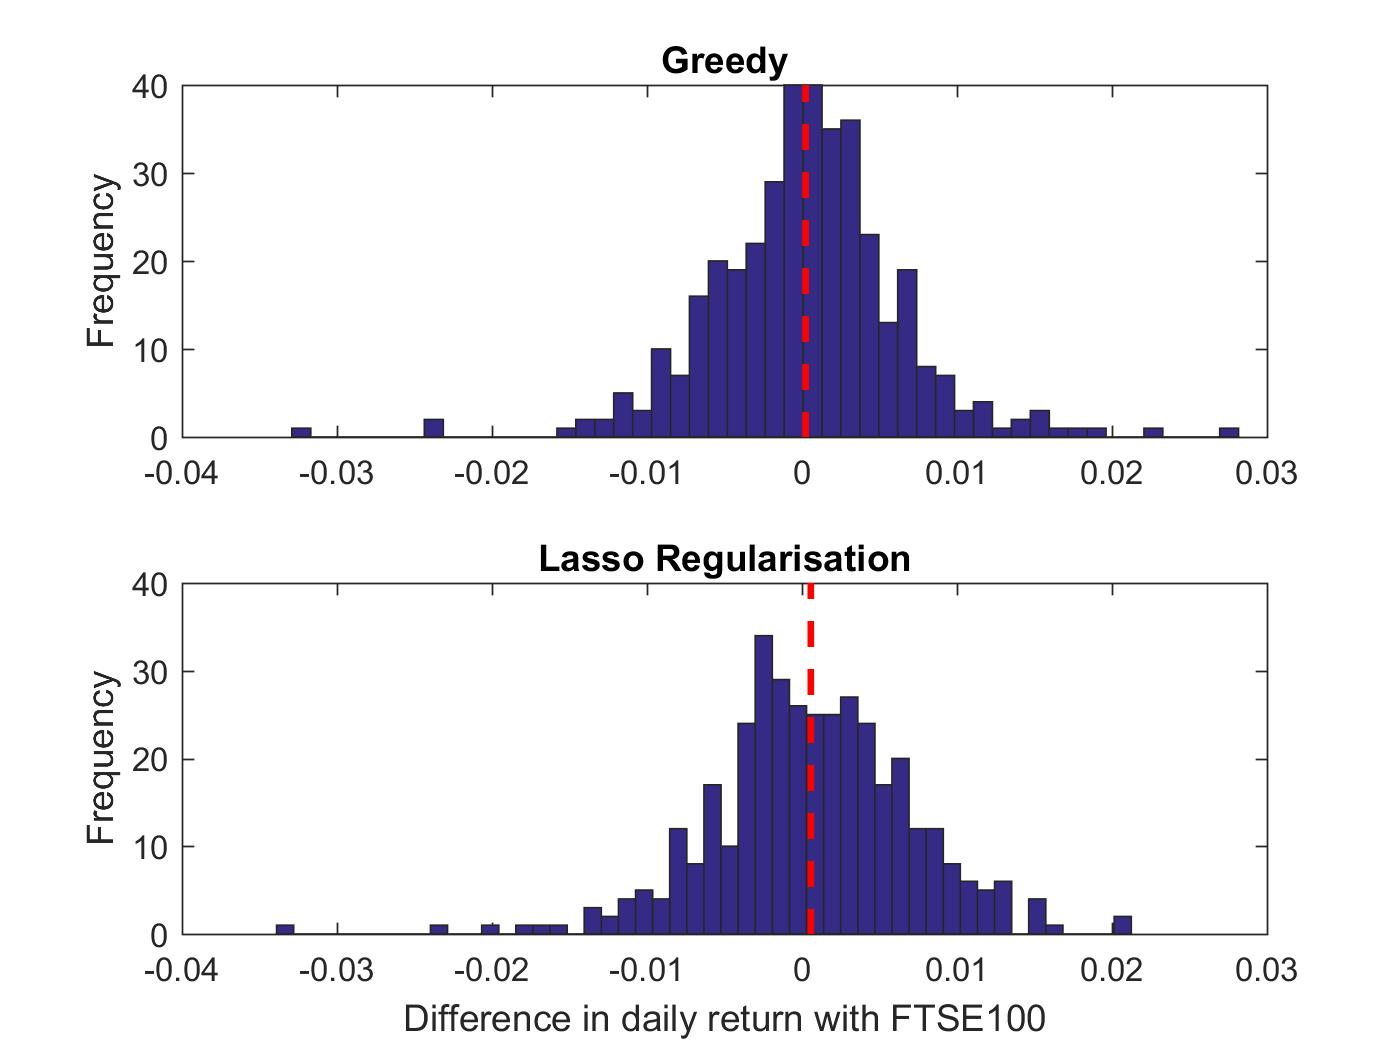
\includegraphics[width=\linewidth]{indexTracking.jpg}
	\centering
	\caption{Difference in daily return between index tracking strategies and the FTSE100 index on the test set. Red dashed line shows the mean error.}
			\label{fig:indexTracking}
\end{figure} 

The average daily difference in returns on the order of $10^-4$. The standard deviation of returns in the FTSE100 is $7 \times 10^-3$. Table \ref{tab:1} and figure \ref{fig:indexTracking} show the ability for the trackers to match the index. The daily standard deviation in the errors is of order $10^-2$ bigger than the expected daily change in the index so both trackers do not necessarily track the FTSE well on a daily basis even on the test set. However they are optimised to minimise the average total error and do this well ($<10\% index \sigma$). 

The Lasso regularisation is much more finely tuned to the test set with lower average error but this appears to result in over-fitting as the error on the test set is greater than the greedy algorithm. In this case that isn't a bad thing as it results in greater returns.

Overall the purpose of tracking indexes is to produce a strong diversified portfolio with an emphasis on reducing risk. To see if these tracking methods can compete on this front we consider their performance metrics out of sample and compare them to the FTSE index and 1/N portfolio. 

The FTSE index performs significantly worse in terms of Sharpe value and return than the 1/N strategy (N=30) however this is at the expense of risk. The FTSE index has the lowest risk of any of the portfolios measured, this is likely due to being able to diversify into 100 assets whereas for our other strategies we have used a sample of 30. The asset tracking algorithms performance change only slightly when trying to track the FTSE or the 1/N strategy and is quite close to the index in value. Considering the performance increase you get in return is significant.  

The purpose of index based portfolios is to minimise risk. In this sense the FTSE index is much better at achieving this than the 1/N strategy. The tracking algorithms get closer to this point under the a low cardinality constraint. The greedy algorithm gives lower risk while the lasso seems to achieve higher returns / Sharpe values. Which of these you choose to use would therefore depend on risk aversion. 
    
\begin{table}
\begin{tabular}{|r|c|c|c|}
\hline
& $\mu$ & $\sigma$ & Sharpe \\
& $10^-3$ & $10^-3$ & $10^-3$ \\
\hline
Greedy & 0.41 & 8.72 & 45.3 \\
Lasso & 0.75 & 10.86 & 67.8 \\
FTSE-100 & 0.18 & 7.03 & 23.5 \\
1/N & 15.78 & 219.3 & 72.0 \\
Greedy (1/N) & 0.41 & 8.72 & 45.3 \\
Lasso (1/N) & 0.81 & 11.79 & 67.7 \\
\hline
\end{tabular}
\caption{Performance metrics of different portfolio optimisation strategies and trackers on the testing set.}
\label{tab:2}
\end{table}
    
\section{Transaction Costs}
In the previous section we saw how fixed cost transaction costs can be modelled with lasso regularisation. This effectively models the behaviour of small scale portfolios where the fixed costs are dominant however for large organisations linear transaction costs are dominant and fixed costs can be largely ignored. Lobo et al. considers linearly modelled transaction costs while optimising changes to portfolios and including other convex constraints: Budget, short selling, variance, diversification and shortfall risk constraints. 

Including a fixed transaction cost results in a non-convex function solving which is NP hard and must be sub-optimally approximated. Simplifying to two convex linear equations which can be optimised with quadratic programming. The transaction costs associated with changing portfolio weights from $\mathbf{w}$ to $(\mathbf{w + x})$:

\[
    \phi_i(x_i)= 
\begin{cases}
    \alpha_i^+x_i,& \text{if } x_i\geq 0\\
    -\alpha_i^-x_i,              & \text{if } x_i\leq 0
\end{cases}
\]

Where $\alpha_i^+/\alpha_i^-$ are the cost rates for buying and selling each asset respectively. 

On top of this model of transaction fees any number of convex constraints can be built under the principle that "If any number of convex transaction costs and convex constraints are combined, the resulting problem is convex."\cite{Lobo}.

\subsection{Example}
Consider the example below, which tries to maximise the expected return under 4 constraints: The budget constraint; a constraint to prevent negative sales or purchases; a limit for the amount of short selling allowed on any one asset and two shortfall constraints which limit the probability of loosing $(1-W_1^{low})$ and $(1-W_2^{low})\%$ of total wealth to $\eta_1$ and $\eta_2$ respectively.

The budget constraint is the idea that the changes in the portfolio must be self-financed so no money goes into or out of the portfolio as a whole, including a risk-less asset this produces an inequality. Managers may want to pursue this constraint to limit their exposure to risk and prevent a money sink portfolio which needs to be propped up with additional funds constantly. 

The short selling constraint sets a limit on how much short selling is permitted for each asset. Short selling is inherently more dangerous and should be limited since the risk of loss is potentially infinite. 

The shortfall risk constraints also try to limit risk by setting acceptable probabilities for different losses. I.e. set the lowest value at return that is acceptable. Short-selling and budget constraints are linear but the shortfall constraint is a second order cone as the inequality is the euclidean distance ($l_2$ norm), which produces a circular boundary projected into a cone but the linear term.      

\begin{align}
\begin{split}
\text{maximise  } &\bar{a}^T(w+x^+-x^-) \\
\text{subject to  } &\mathbf{1}^T(x^+-x^-)+ \sum^n_{i=1}(\alpha_i^+x_i^++\alpha^-_ix^-_i) \leq 0 \\
&x_i^+ \geq 0, x_i^- \geq 0, i = 1,...,n \\
&w_i+x_i^+ - x_i^- \geq s_i, i = 1,...,n \\
& \Phi^{-1}(\eta_j)||\Sigma^{1/2}(\omega+x^+-x^-)|| \\ \: &\leq \bar{a}^T(\omega+x^+-x^-) - W_j^{low}, j = 1,2
\end{split}
\label{eq:8}
\end{align}

In order to implement this into the work in previous sections the CVX optimisation steps of the Naive\_MW algorithm can be adjusted to fit in the additional constraints, with syntax which follows (\ref{eq:8}). The code for the first of these optimisation methods is as follows:
\begin{lstlisting} 
cvx_begin
variable MaxReturnWts(N_assets) nonnegative
variable SalesWts(N_assets) nonnegative
variable BuyWts(N_assets) nonnegative
maximise(MaxReturnWeights' * ERet)
subject to
	MaxReturnWeights' * ones(N_assets,1) == 1;
	MaxReturnWts == BuyWts - SalesWts;        
	%Budget constraint    
    (SalesWts - BuyWts)' * ones(N_assets,1) + ...
    BuyCost' * BuyWts + SalesCost' * SalesWts <= 0;
	% Short selling limit    
    min(MaxReturnWeights' * ones(N_assets,1) >= s;
	% Shortfall constraints	
	norm(sqrt(C)*MaxReturnWts) ...
	<= Eret * MaxReturnWts - W_low(1);
	norm(sqrt(C)*MaxReturnWts) ...
	<= Eret * MaxReturnWts - W_low(2);     
cvx_end
\end{lstlisting} 
\section{Conclusion}
In conclusion we have seen how the Mean-Variance Frontier can be used to generate optimised portfolios when the mean and covariance of stocks is known. However Because these properties aren't stable and the performance of the frontier is chaotic estimation error causes large performance issues with these portfolios, leading to naive approaches being more favourable. 

For more passive portfolios indexes are a good way to diversify however for small scale investors fixed costs must be taken into account and approximations of indexes have to be made in order to minimise these costs. Two methods of achieving this are using a greedy algorithm which has lower out of sample variance or lasso regularisation which has higher out of sample return. 

For large scale investors fixed costs can be ignored and linear costs must be modelled instead, alongside other possible convex constraints. Matlab's CVX package can easily adapt to these additional constraints and provide optimised portfolios for these scenarios. 

\begin{thebibliography}{9}
\bibitem{Portfolio}
  H. Markowitz,
  "Portfolio selection",
  The Journal of Finance, 
  vol 7, 
  no. 1, 
  pp. 77 - 91, 
  (1952).
\bibitem{TextBook}
  P. Brandimarte,
  "Numerical Methods in Finance and Economics",
  Wiley, 
  (2006).
\bibitem{VsNaive}
  V. DeMiguel, L. Garlappi, and R Uppal, 
  "Optimal versus naive diversification: How inefficient is the 1/n portfolio strategy?",
  The Review of Financial Studies, 
  Vol 22,
  no. 5, 
  pp. 1915 - 1953, 
  (2009).
\bibitem{Regularisation}
  J. Brodie, I. Daubechies, C. De Mol, D. Giannone, and I. Loris, 
  "Sparse and stable Markowitz portfolios", 
  PNAS, 
  vol. 106, 
  no. 30,
  pp. 12267-12272, 
  (2009).
\bibitem{Lobo}
  M. Lobo, M. Fazel and S. Boyd, 
  "Potfolio optimization with linear and fixed transaction costs", 
  Annals of Operations Research, 
  vol. 152, 
  no. 1, 
  pp. 341 - 365, 
  (2007).
\bibitem{CVX}
  Grand, Micheal, Stephen Boyd, and Yinyu Ye,
  "CVX: Matlab software fore disciplined convex programming.",
  (2008).
\bibitem{Matlab}
  "MATLAB and Financial Toolbox",
   Release 2015b, 
   The MathWorks, Inc., 
   Natick, 
   Massachusetts, United States.


\end{thebibliography}
\end{document}
